% !TeX root = ./presentazione.tex
% !TeX encoding = UTF-8 Unicode
% !TeX spellcheck = it_IT
% !TeX program = arara
% !TeX options = --log --verbose --language=it "%DOC%"

% arara: lualatex: { interaction: batchmode }
% arara: lualatex: { interaction: nonstopmode, synctex: yes }

\documentclass[
  usepdftitle=false,
  % notes,
  bigger,
  aspectratio=169,
  lualatex,
  % handout,
  italian
]{beamer}

\usepackage{pgfpages}
\usepackage{fontspec}
\defaultfontfeatures{Ligatures={TeX}}
\usepackage[
  output-decimal-marker={,},
  binary-units
]{siunitx}
\usepackage[%
  strict=true,
  autostyle=true,
  english=american,
  italian=guillemets
]{csquotes}
\usepackage{polyglossia}
\setmainlanguage[babelshorthands]{italian}
\setotherlanguage[variant=american]{english}
\usepackage{graphicx}
% \usepackage{svg}
% \usepackage{tikz}
% \usepackage{multimedia}
\usepackage{media9}
% \usepackage{minted}
\usepackage[
  subrefformat=parens,
  labelformat=parens
]{subcaption}
\usepackage{caption}
\usepackage{adjustbox}
\usepackage{microtype}

\hypersetup{%
  pdftitle={Progettazione di una piattaforma web per la simulazione di programmi aggregati},
  pdfauthor={Niccolò Maltoni},
  pdfsubject={La programmazione aggregata è un approccio innovativo nato in tempi recenti per far fronte alla necessità di un punto di vista nuovo nella programmazione di sistemi distribuiti. In particolare, basandosi sull'impianto teorico del field calculus, negli ultimi anni sono stati realizzati, da parte dell'Università di Bologna, linguaggi e framework innovativi per la sua applicazione in contesti d'uso reale: Protelis e ScaFi. La principale criticità che mina la diffusione di questo tipo di linguaggi è legata alla configurazione del sistema per l'esecuzione: è infatti necessario avere a disposizione una rete, reale o fisica, di dispositivi per l'esecuzione del codice e, soprattutto in contesto didattico, la necessità di dispiegare un certo numero di dispositivi o configurare un simulatore può costituire un ulteriore gradino di complessità. Lo scopo di questa tesi è progettare una piattaforma web che permetta di realizzare semplici programmi aggregati senza configurazione alcuna. È stato realizzato un sistema composto da un server esecutore, che si avvale del simulatore Alchemist per eseguire il codice Protelis, e da un'applicazione web in React che permetta la scrittura del codice e il monitoring dell'esecuzione.},
  pdfkeywords={Aggregate computing, Aggregate programming, Protelis, Applicazione web, Simulazione},
  pdfpagemode={UseNone},
  hidelinks,
  hypertexnames=false,
  linktoc=all,
  unicode=true,
  pdftoolbar=false,
  pdfmenubar=false,
  plainpages=false,
  breaklinks,
  pdfstartview={Fit},
  pdflang={it}
}

\usetheme{Boadilla}
\usecolortheme{beaver}
\setbeameroption{hide notes} % Only slide
%\setbeameroption{show only notes} % Only notes
%\setbeameroption{show notes on second screen=right} % Both
\setbeamertemplate{note page}[plain]
\beamertemplatenavigationsymbolsempty
\hypersetup{pdfpagemode=UseNone} % don't show bookmarks on initial view
% \setbeamertemplate{items}[triangle]

\title[WebProtelis]{%
  Progettazione di una piattaforma web per la\\simulazione di programmi aggregati%
}

\subtitle{Tesi in Pervasive Computing}

\author[Niccolò~Maltoni (0000840825)]{%
  Niccolò~Maltoni%
  \\\small{Matricola: 0000840825}%
  \\\vspace{10pt} \small{Realtore: Prof.~Mirko~Viroli \\Correlatore: Prof.~Danilo~Pianini}
}

\institute[]{Alma Mater Studiorum - Università di Bologna}

\date{19 marzo 2020}

% %% Permette di inserire l'outline prima di ogni sezione
% \AtBeginSection[]{%
%   \begin{frame}<beamer>
%     \frametitle{Outline}
%     \tableofcontents[currentsection]
%   \end{frame}
% }

\begin{document}

  \frame{\titlepage}

  % \begin{frame}<beamer>
  %   \frametitle{Outline}
  %   \tableofcontents
  % \end{frame}

  \addchap{Introduzione}\label{ch:intro}

% Nel corso degli ultimi anni i sistemi informatici hanno avuto uno sviluppo sempre crescente,
Nel corso degli ultimi anni i sistemi informatici hanno avuto uno sviluppo notevole.
Grazie all'incremento della potenza computazionale disponibile a basso costo, alla riduzione delle dimensioni delle unità di calcolo e alla diffusione delle reti wireless,
ormai gli ambienti in cui vive la maggior parte della popolazione sono pervasi di sensori (il cosiddetto \emph{IoT}, Internet delle Cose) e di dispositivi ``smart'' (come smartphone e tablet).

Questo ha portato alla necessità di programmare sistemi distribuiti composti da numerosi dispositivi che devono potersi coordinare tra loro
per poter portare a termine la computazione.

La \emph{programmazione aggregata} è un approccio promettente per lo sviluppo di sistemi di questo tipo.
Tale paradigma è basato sull'impianto teorico del \emph{field calculus} e ha visto negli ultimi anni la realizzazione,
da parte dell'Università di Bologna, di linguaggi e framework innovativi per la sua applicazione in contesti d'uso reale:
\emph{Protelis} e \emph{ScaFi}.

Entrambi si avvalgono della piattaforma JVM per poter essere eseguiti;
come vedremo, questo garantisce numerose proprietà, ma può essere limitante in contesti didattici.
Infatti, la necessità di possedere una rete reale di dispositivi o di configurare un simulatore per l'esecuzione
aggiunge ulteriore complessità per un novizio che voglia approcciarsi alla tecnologia.
Inoltre, non è da ignorare nemmeno la necessità di configurazione di un progetto Gradle o SBT completo per poter realizzare un prototipo minimale.

In tempi recenti anche il web è maturato molto:
l'evoluzione tecnologica ha permesso di realizzare applicazioni utilizzabili tramite browser con livelli di complessità comparabili alle controparti desktop,
senza il carico aggiuntivo, dal punto di vista dell'utente, dell'installazione e della configurazione.
Inoltre, servizi complessi possono non dipendere esclusivamente dalle risorse computazionali dei dispositivi dell'utente,
bensì sfruttarle solo quando necessario, appoggiandosi alla potenza computazionale di un server di backend per le operazioni più complesse.

Si è dunque ritenuto utile realizzare un sistema web semplice e immediato da usare che permetta di abbozzare esempi di codice aggregato
(Protelis, nel prototipo implementato per questa tesi) e poterlo eseguire senza disporre di una rete di dispositivi o di un simulatore configurati per lo scopo.
In particolare, si è deciso di propendere per l'implementazione di un backend reattivo su piattaforma JVM che esegue, su una rete di dispositivi simulata tramite il simulatore Alchemist, il codice inviato da un client.
Il client è una \emph{Single-Page Application} statica che permette lo sviluppo di codice direttamente dal browser e comunica con il server tramite bus di eventi.

\bigskip

Il documento è suddiviso in tre \nameCrefs{part:background} principali.

Nella~\Cref{part:background} viene fatta una disamina del contesto nel quale l'elaborato di tesi va a inserirsi.
In particolare, nel~\Cref{ch:motivations} vengono esaminate più nel dettaglio le ragioni per le quali il progetto è stato realizzato,
con particolare attenzione allo stato dell'arte e a possibili soluzioni a problemi simili.
Nel~\Cref{ch:aggregate} del documento viene fatta un'introduzione alla programmazione aggregata, con particolare attenzione all'impianto teorico su cui si basa e ai linguaggi ad essa collegati.
Nel~\Cref{ch:web} viene invece fatta riportato il risultato della fase di studio dello stato dell'arte in merito allo sviluppo di sistemi web,
con particolare attenzione ai linguaggi che permettono la realizzazione di applicazioni frontend in esecuzione sui browser degli utenti.

Nella~\Cref{part:contribution} viene analizzato il processo di progettazione del sistema a cui questo elaborato di tesi si riferisce e di sviluppo del prototipo.
Ciascuna fase del processo è descritta in un \nameCref{ch:requirements} dedicato.

Infine, nella~\Cref{part:conclusion} vengono raccolti i risultati del processo di sviluppo (\Cref{ch:evaluation}), presentate le prospettive future (\Cref{ch:future}) ed enunciate brevemente le considerazioni finali (\Cref{ch:considerations}).

  \section{Background}
    \subsection{Stato dell'arte}

      \begin{frame}{\insertsectionhead}{\insertsubsectionhead}
        \begin{columns}
          \begin{column}{.7\textwidth}
            \begin{block}{Programmazione aggregata}
              La programmazione aggregata costituisce un'alternativa all'approccio ``classico'' volta a semplificare la progettazione, creazione e manutenzione di sistemi distribuiti complessi.
            \end{block}

            \begin{block}{Linguaggi}
              I principali linguaggi di programmazione aggregata sono:

              \begin{itemize}[<+(1)->]
                \item ScaFi
                \item Protelis
              \end{itemize}
            \end{block}
          \end{column}
          \begin{column}{.25\textwidth}
            \begin{figure}
              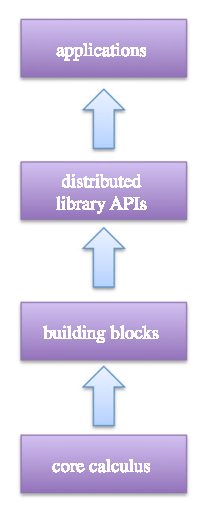
\includegraphics[height=.7\textheight]{res/fig/stack-partial.eps}
            \end{figure}
          \end{column}
        \end{columns}
      \end{frame}

      \begin{frame}{\insertsectionhead}{\insertsubsectionhead}
        \begin{columns}
          \begin{column}{.8\textwidth}
            \begin{block}{Protelis}
              \begin{itemize}[<+->]
              \item
                  Linguaggio di programmazione basato sul paradigma aggregato fortemente influenzato da \emph{Proto}
                \item
                  Incorpora le principali funzionalità di computazione spaziale della programmazione aggregata
                \item
                  Possiede una sintassi più simile ai linguaggi strutturati tradizionali come C o Java
                \item
                  È \emph{Java-hosted}
                  \begin{itemize}
                    \item richiede un ambiente JVM in cui eseguire l'interprete
                  \end{itemize}
              \end{itemize}
            \end{block}
          \end{column}
          \begin{column}{.15\textwidth}
            \begin{figure}
              
\includegraphics[width=\textwidth]{../res/fig/protelis-logo.png}
            \end{figure}
          \end{column}
        \end{columns}
      \end{frame}

    \subsection{Problematica}

    \begin{frame}{\insertsectionhead}{\insertsubsectionhead}
      \begin{columns}
        \begin{column}{.6\textwidth}
          \begin{alertblock}{\insertsubsectionhead}
            \begin{itemize}
              \item<1->
                Il linguaggio richiede una rete di dispositivi su cui eseguire:
                \begin{itemize}
                  \item<2-> rete fisica
                  \item<3-> NASA WorldWind
                  \item<4-> ProtelisVM
                  \item<5-> Alchemist
                \end{itemize}
            \end{itemize}
          \end{alertblock}
        \end{column}
        \begin{column}{.35\textwidth}
          \begin{figure}
            \centering
            \only<2>{%
              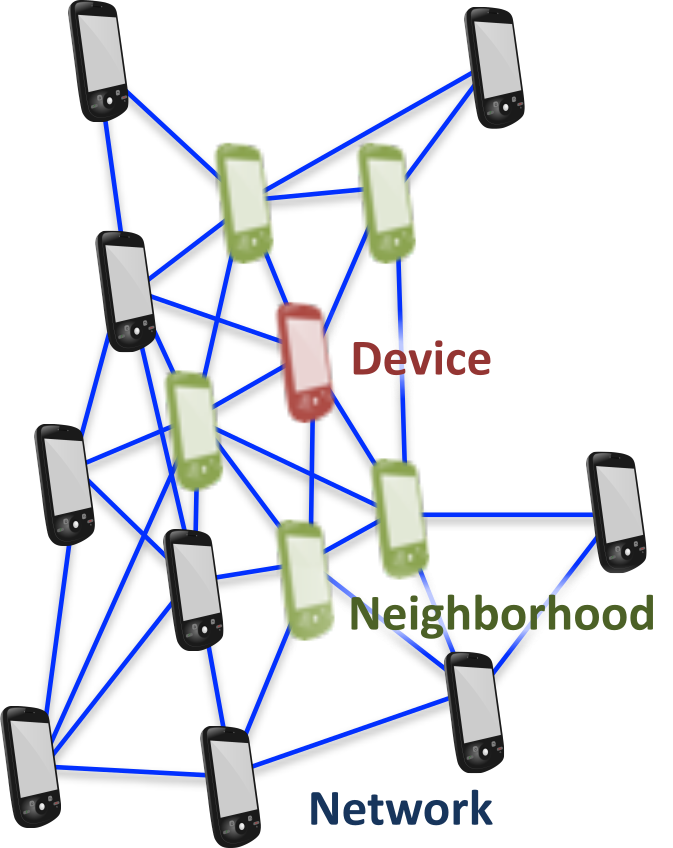
\includegraphics[width=.8\textwidth]{res/fig/network.png}%
            }%
            \only<3>{%
              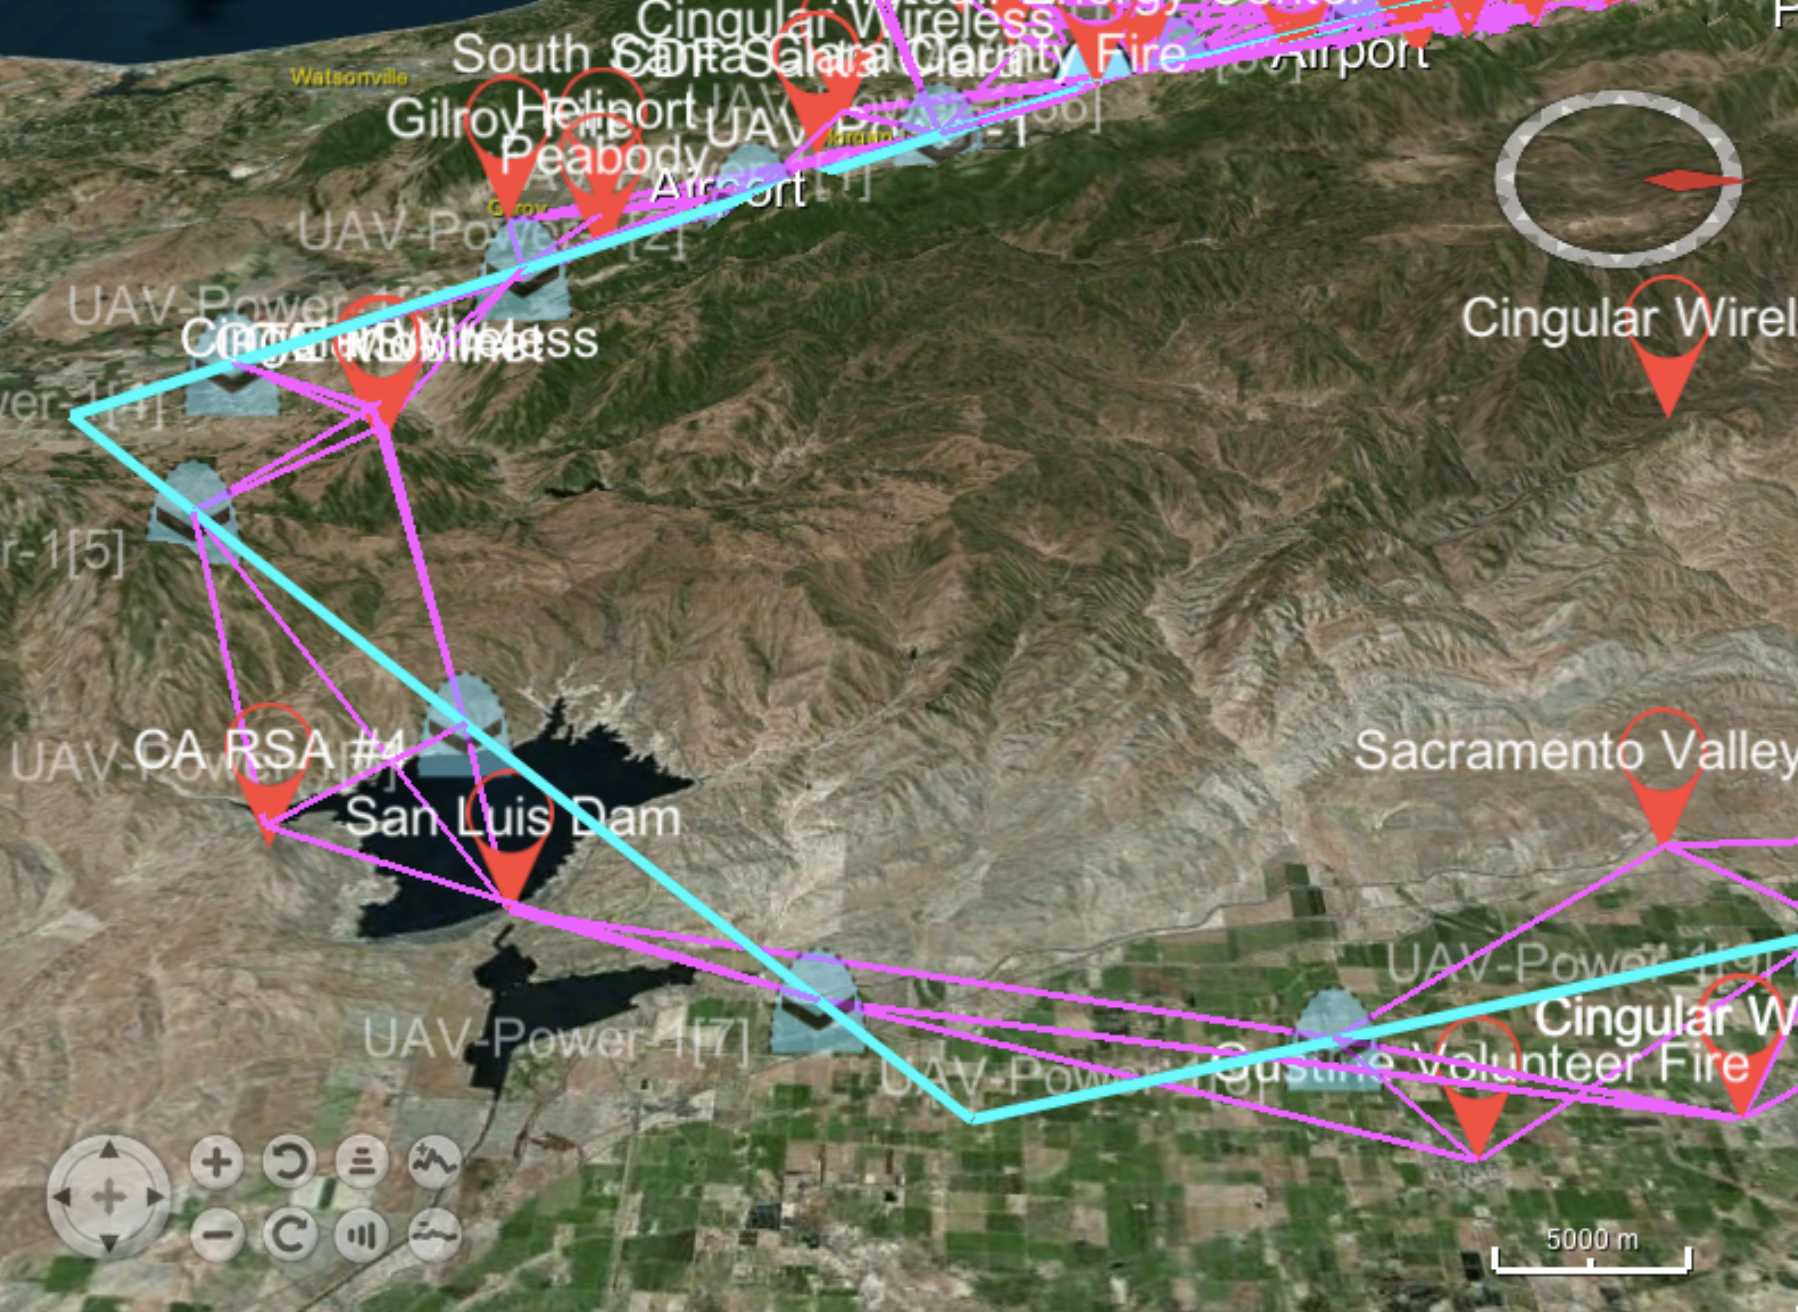
\includegraphics[width=.85\textwidth]{res/fig/nasaworldwind.png}%
            }%
            \only<4>{%
              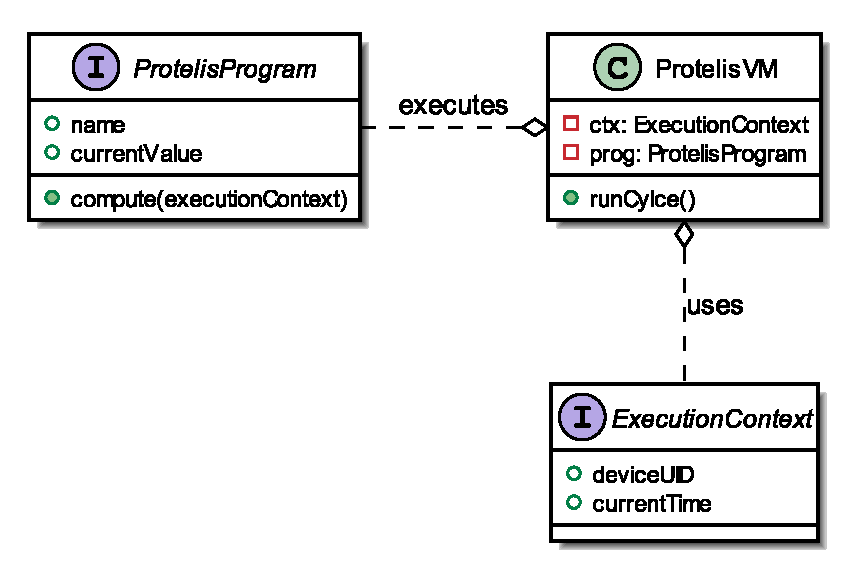
\includegraphics[width=.85\textwidth]{res/uml/protelis-vm.eps}%
            }%
            \only<5>{%
              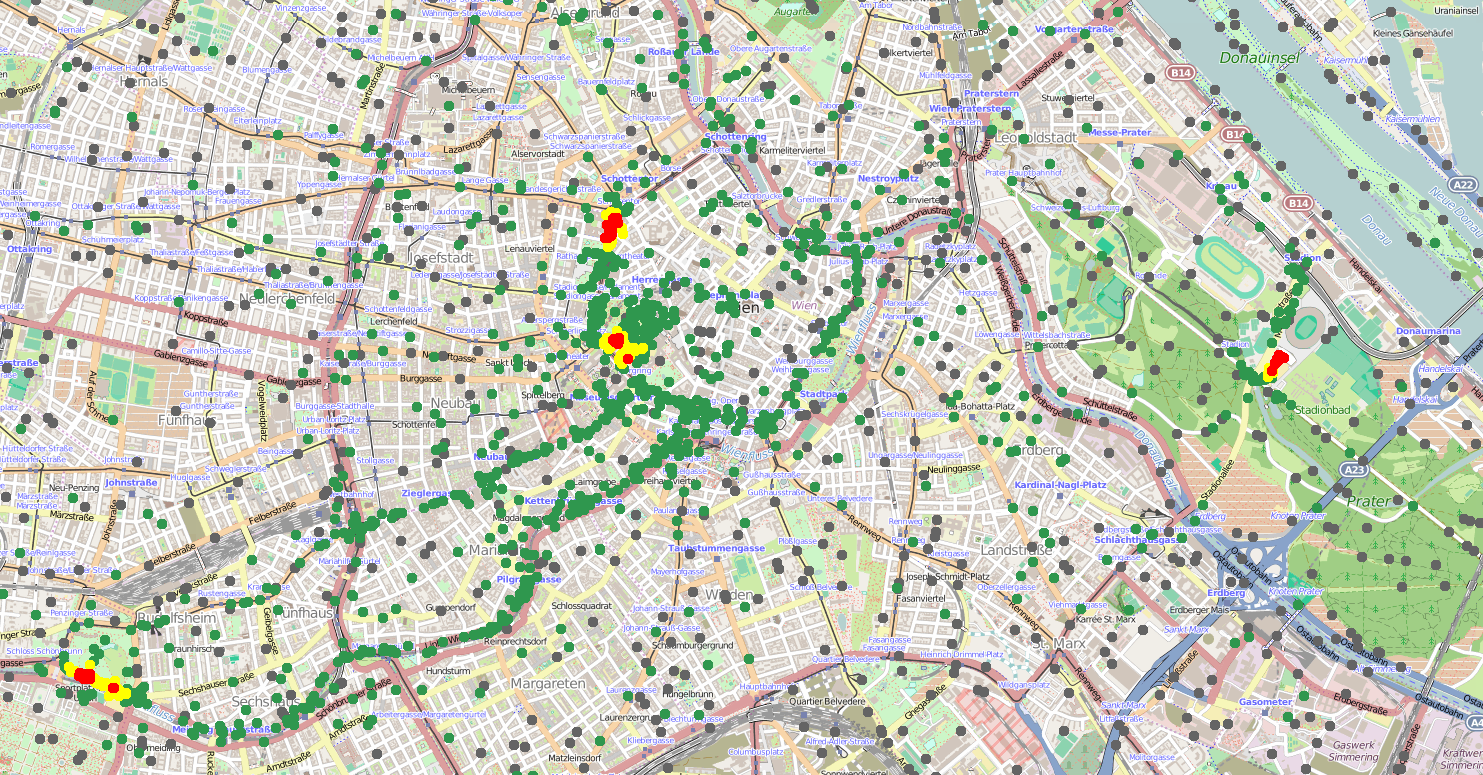
\includegraphics[width=.85\textwidth]{res/fig/alchemist.png}%
            }%
            \only<6>{%
              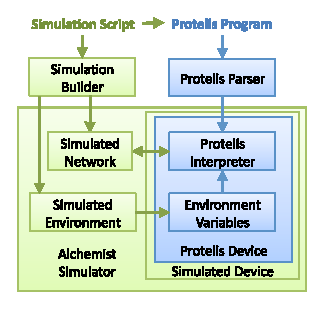
\includegraphics[width=.8\textwidth]{res/fig/protelis-alchemist-arch.eps}%
            }%
          \end{figure}
        \end{column}
      \end{columns}
    \end{frame}

    \subsection{Requisiti e casi d'uso}

    \begin{frame}{\insertsectionhead}{\insertsubsectionhead}
      \begin{columns}
        \begin{column}{.5\textwidth}
          \begin{block}{Requisiti}
            \begin{itemize}
              \item
                Progettare un sistema che permetta di iniziare a utilizzare Protelis con meno configurazioni possibile.
                \begin{itemize}
                  \item nessun build-script
                  \item nessuna rete o simulatore
                \end{itemize}
              \item
                L'utente si assume essere inesperto della piattaforma
                \begin{itemize}
                  \item l'interfaccia deve essere semplice e immediata
                \end{itemize}
              \item La piattaforma dovrebbe essere accessibile tramite browser
            \end{itemize}
          \end{block}
        \end{column}
        \begin{column}{.45\textwidth}
          \begin{figure}
            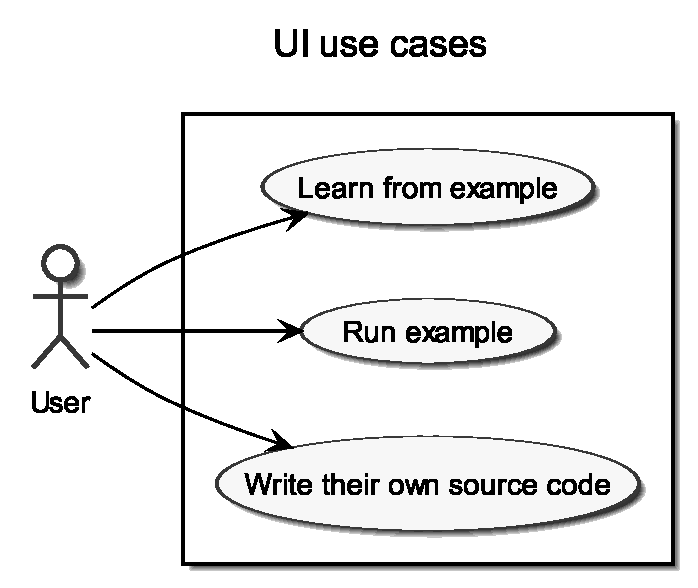
\includegraphics[width=\textwidth]{res/uml/use-cases-frontend.eps}
          \end{figure}
        \end{column}
      \end{columns}
    \end{frame}

    \begin{frame}{\insertsectionhead}{\insertsubsectionhead}

      \begin{block}{Analisi del problema}
        \begin{itemize}
          \item
            non è possibile eseguire un interprete Protelis all'interno della sandbox un browser
            \begin{itemize}
              \item le Java applet sono deprecate da tempo
            \end{itemize}
          \item
            è necessario suddividere l'architettura in due componenti
            \begin{itemize}
              \item un server che espone API per l'esecuzione del codice
              \item un'interfaccia Single-Page accessibile tramite browser
            \end{itemize}
        \end{itemize}
      \end{block}

      \begin{figure}
        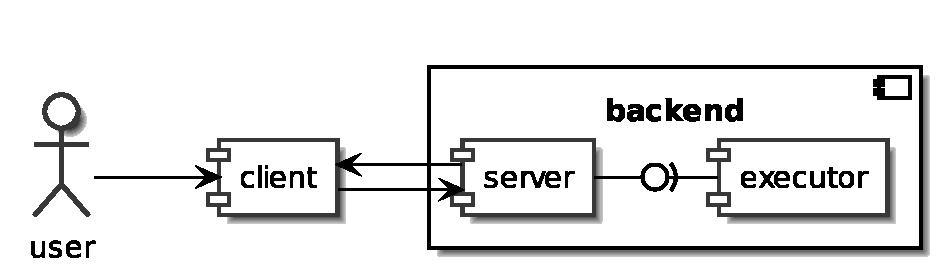
\includegraphics[width=.71\textwidth]{../res/uml/architecture-design.eps}
      \end{figure}
    \end{frame}

  \section{WebProtelis}

  \begin{frame}{\insertsectionhead}
    \begin{figure}
      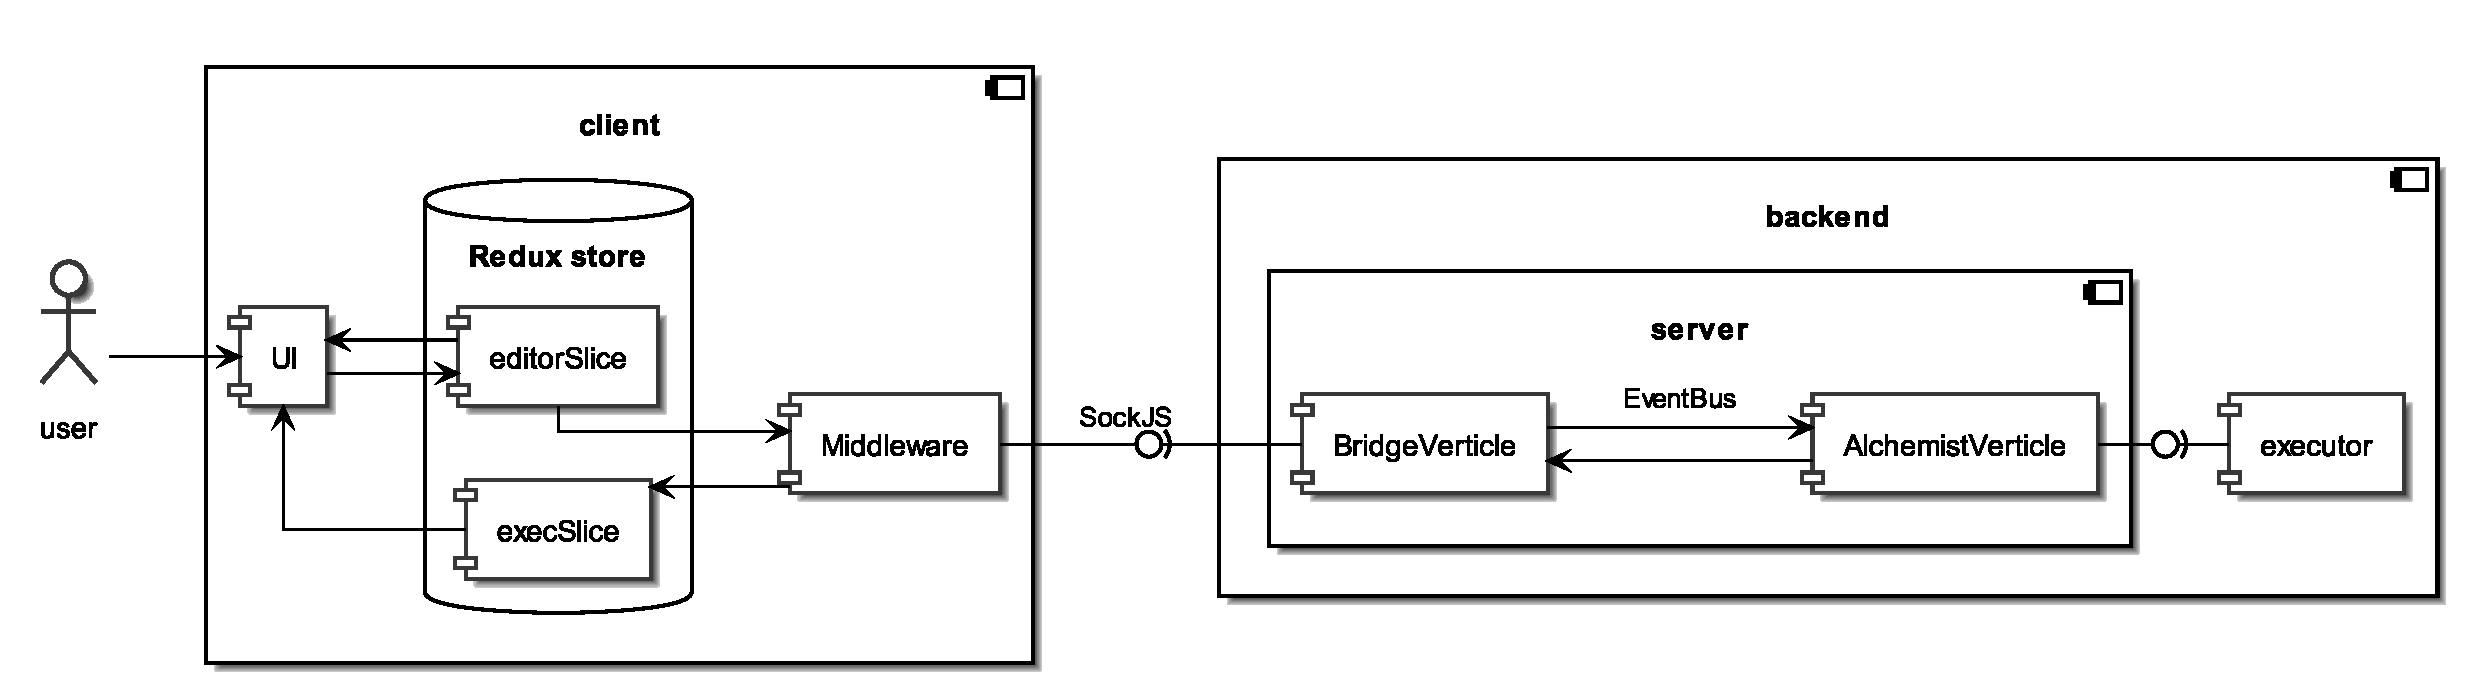
\includegraphics[width=\textwidth]{res/uml/architecture-design-detail.eps}
    \end{figure}
  \end{frame}

  \subsection{Progettazione del server}

    \begin{frame}{\insertsectionhead}{\insertsubsectionhead}

      % \begin{columns}
        % \begin{column}{.55\textwidth}
          \begin{block}{Servizi offerti}
            Il backend mette a disposizione due funzionalità principali:
            \begin{itemize}
              \item API per la comunicazione remota
              \item esecutore del codice Protelis
            \end{itemize}
          \end{block}
        % \end{column}
        % \begin{column}{.4\textwidth}
          \begin{figure}
            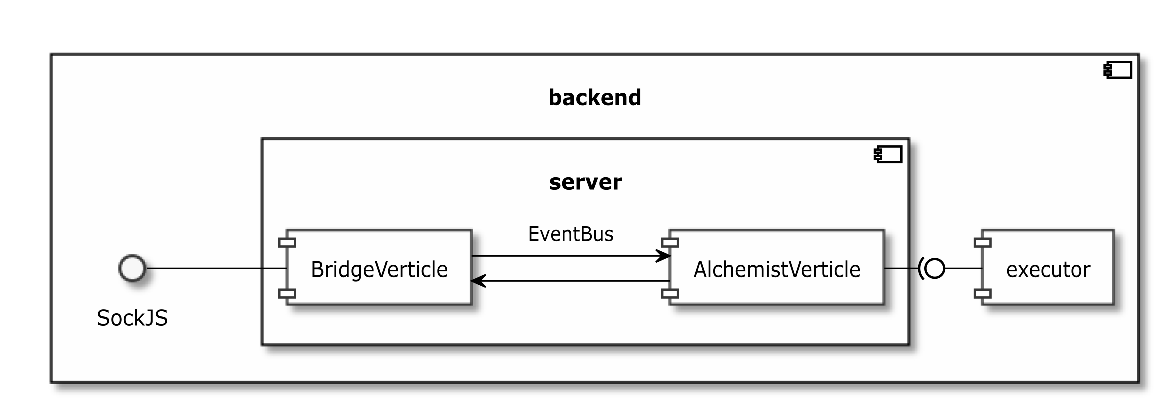
\includegraphics[width=.67\textwidth]{res/uml/architecture-design-server.eps}
          \end{figure}
        % \end{column}
      % \end{columns}
    \end{frame}

    \begin{frame}{\insertsectionhead}
      \framesubtitle{\insertsubsectionhead}

      \begin{columns}
        \begin{column}{.8\textwidth}
          \begin{block}{Vert.x}
            \strong{Vert.x} è un framework applicativo reattivo e event-driven per JVM.

            Caratteristiche principali:
            \begin{itemize}
              \item<2-> reattivo e basato su pattern Multi-Reactor
              \item<3-> supporto a costrutti \emph{actor-like} detti \strong{Verticle}
              \item<4-> supporto a comunicazione tramite EventBus
            \end{itemize}

            % Del modello architetturale messo a disposizione dal framework, è stato considerato interessante il concetto di \emph{Verticle}:
            % esso è un'astrazione, simile al pattern ad attori ma non considerato pienamente aderente al modello teorico dalla stessa documentazione ufficiale,
            % che incapsula un event-loop insieme al suo stato e interagisce tramite gli eventi provenienti da un EventBus.
          \end{block}
        \end{column}
        \begin{column}{.15\textwidth}
          \begin{figure}
            
\includegraphics[width=\textwidth]{res/uml/vertx-logo-big.png}
          \end{figure}
        \end{column}
      \end{columns}

      \begin{block}<5->{Verticle modellati}
        \begin{itemize}
          \item \texttt{BridgeVerticle} gestisce le API attraverso \emph{SockJS} e \emph{EventBus}
          \item \texttt{AlchemistVerticle} costruisce e monitora simulazioni Alchemist per eseguire il codice Protelis
        \end{itemize}
      \end{block}
    \end{frame}

    \subsection{Progettazione del client}

    % \begin{frame}{\insertsectionhead}{\insertsubsectionhead}
    %   \begin{block}{Struttura}
    %     \begin{itemize}
    %       \item<1-> Il client dovrebbe essere una Single-Page Application composta da un editor e da un canvas
    %       \item<2-> Simile a CodeSandbox\onslide<3->{, TypeScript Playground }\onslide<4->{o Overleaf}
    %     \end{itemize}
    %   \end{block}

    %   \begin{figure}
    %     \centering
    %     \only<2>{%
    %       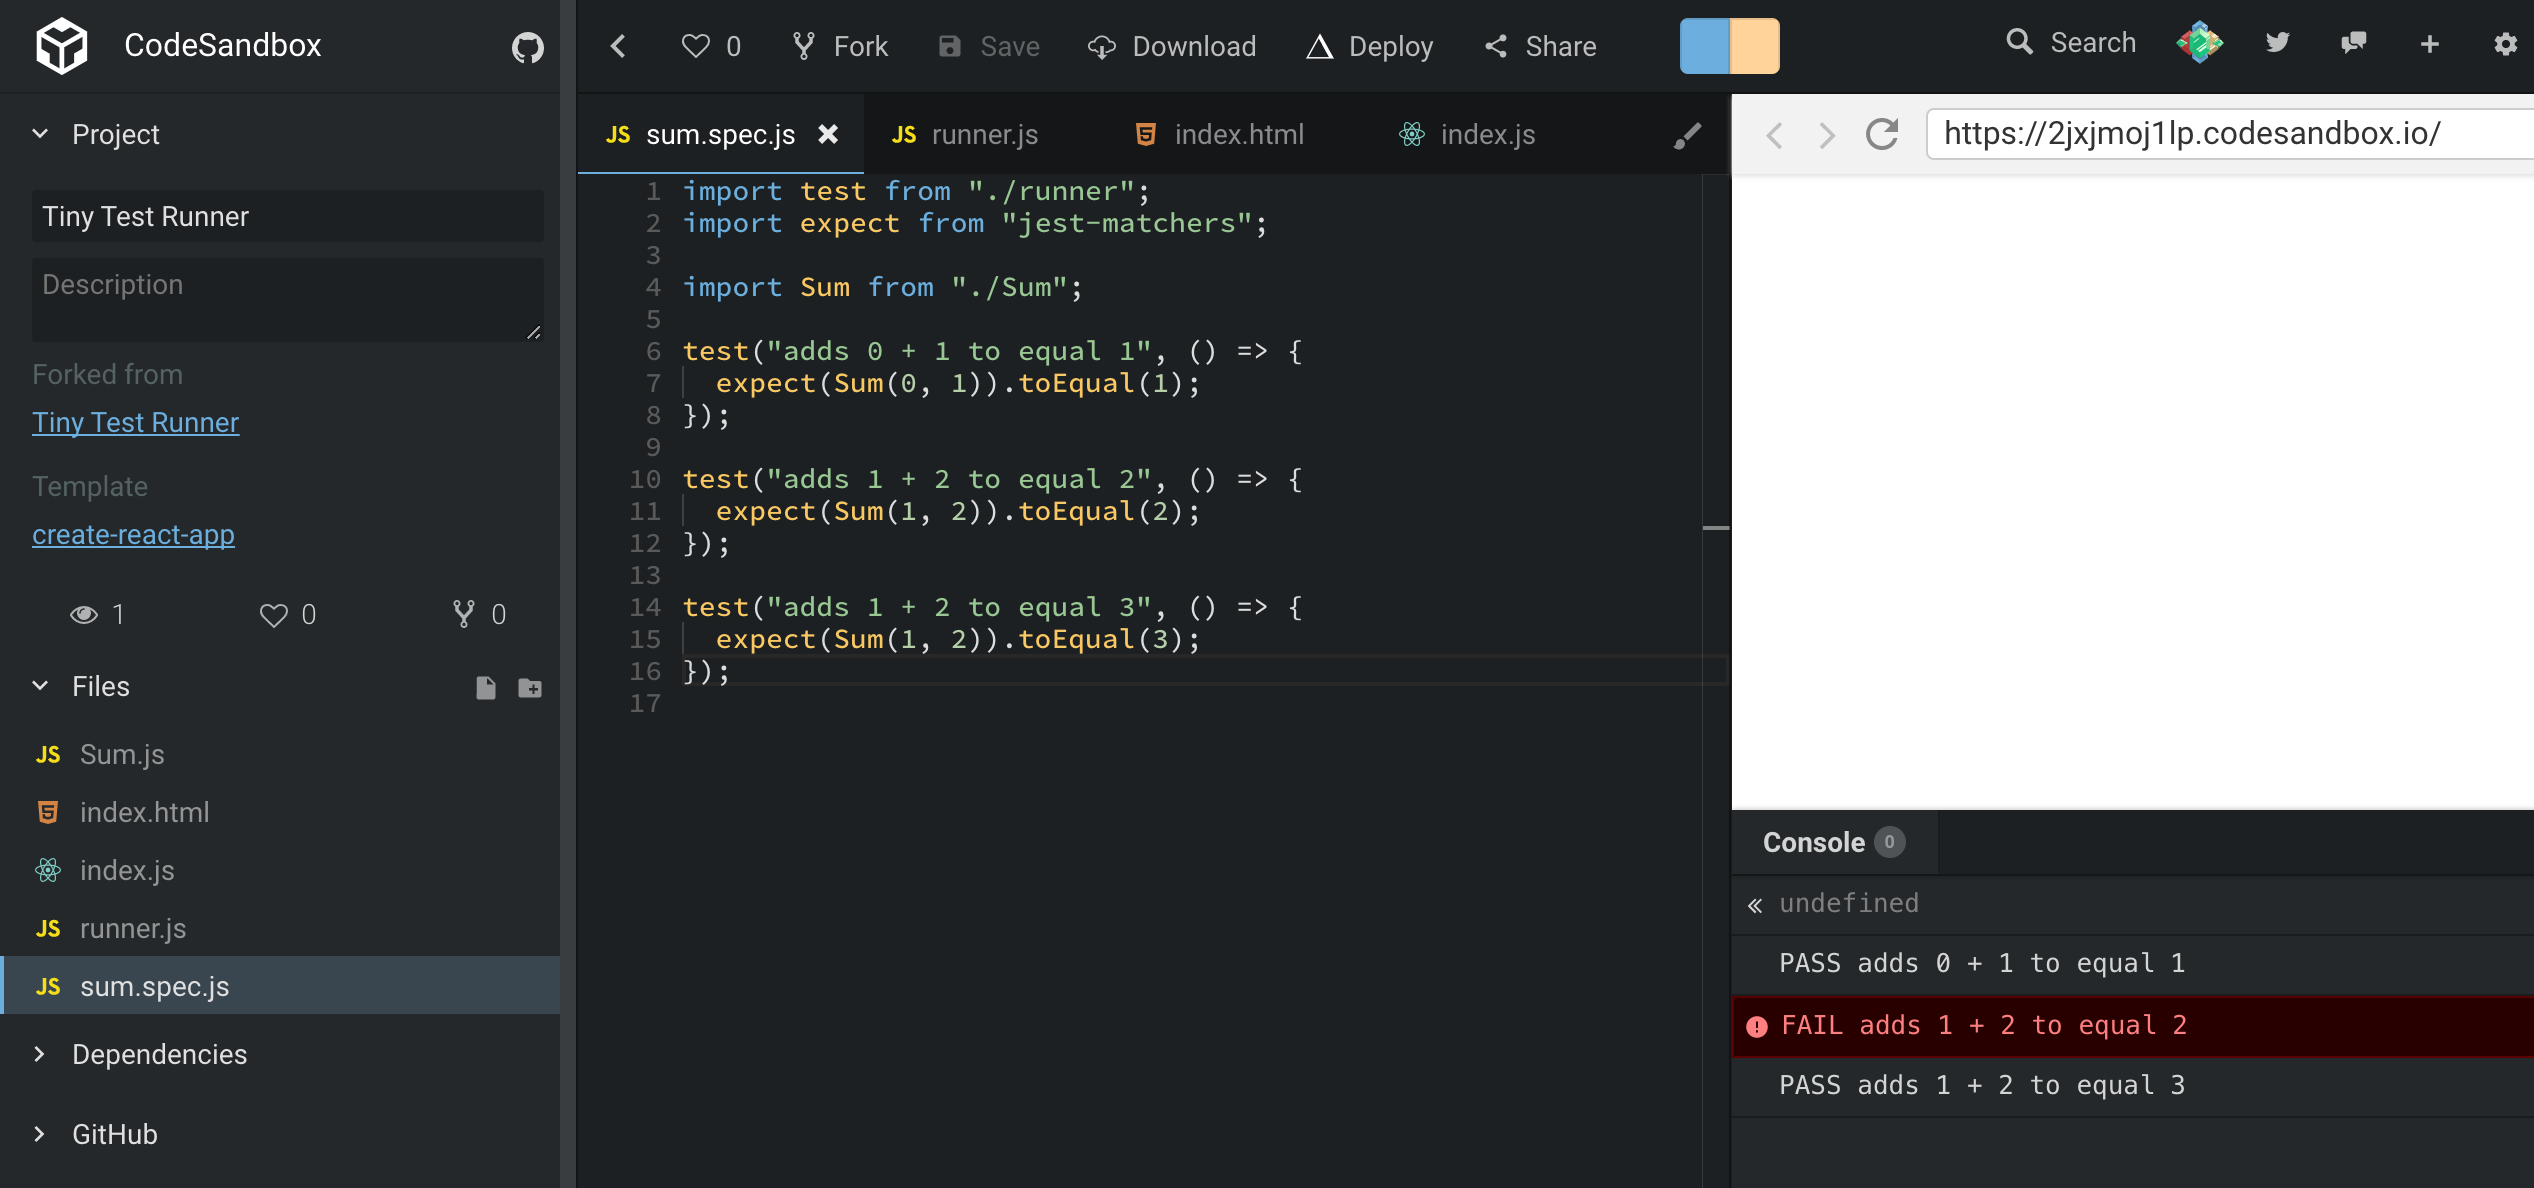
\includegraphics[width=.5\textwidth]{res/fig/codesandbox.png}%
    %     }%
    %     \only<3>{%
    %       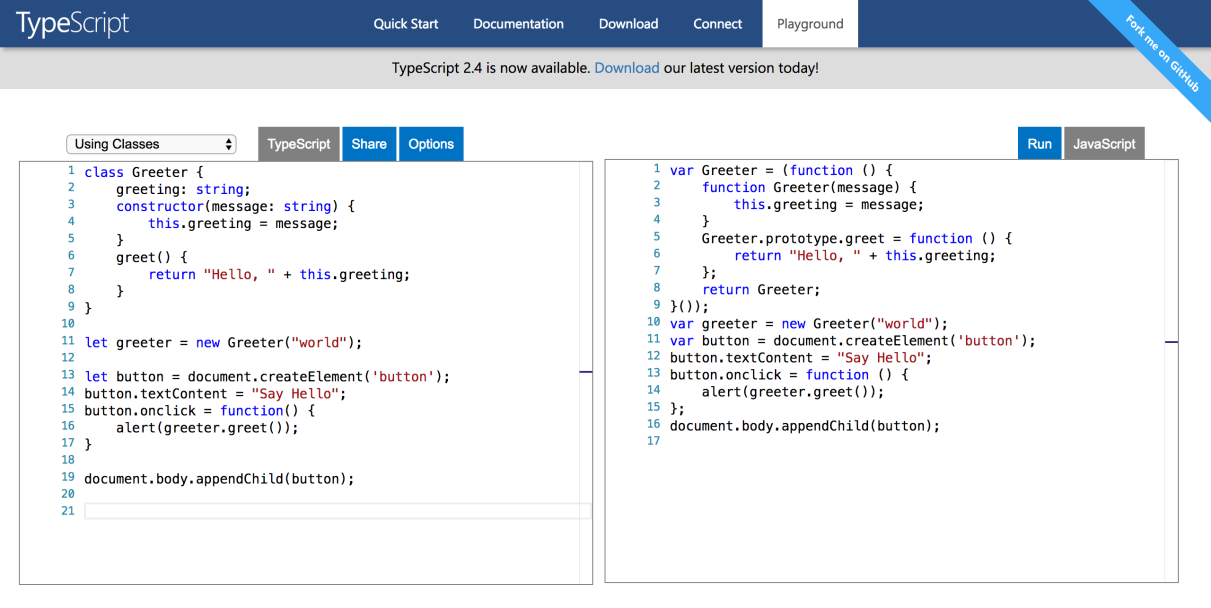
\includegraphics[width=.5\textwidth]{res/fig/typescript-playground.png}%
    %     }%
    %     \only<4>{%
    %       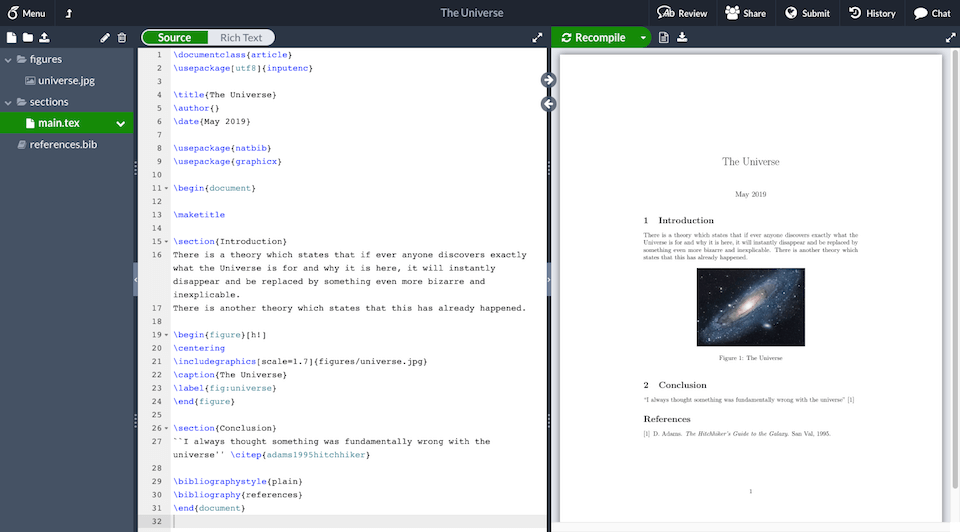
\includegraphics[width=.5\textwidth]{../res/fig/overleaf.png}%
    %     }%
    %   \end{figure}
    % \end{frame}

    % \begin{frame}{\insertsectionhead}{\insertsubsectionhead{}: Mockup}
    %   \centering
    %   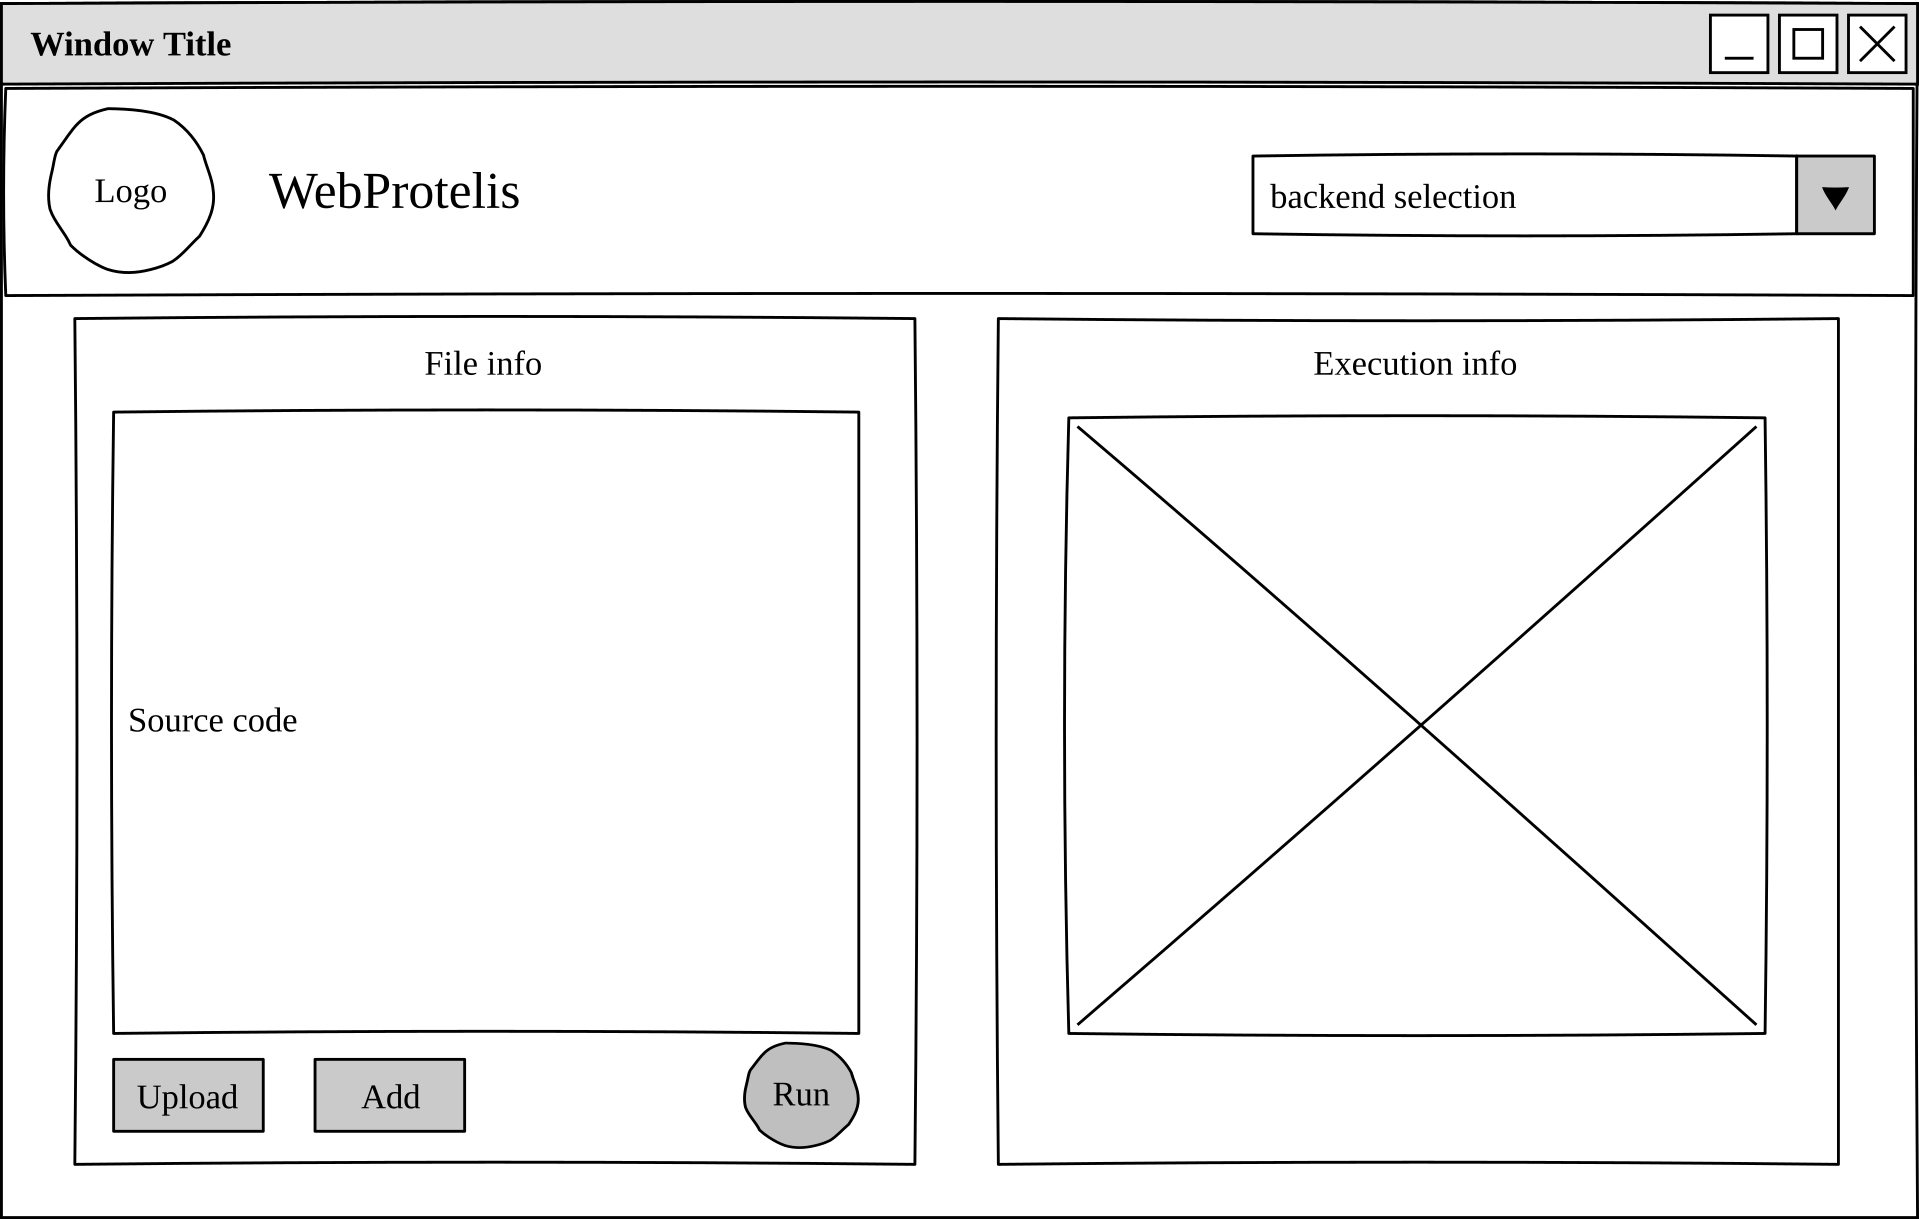
\includegraphics[width=.9\textwidth]{res/fig/gui-actual.png}
    % \end{frame}

    \begin{frame}{\insertsectionhead}{\insertsubsectionhead}
      \begin{columns}
        \begin{column}{.8\textwidth}
          \begin{block}{Framework}
            \begin{itemize}
              \item
                Per l'implementazione è stato scelto \strong{React}
                \begin{itemize}
                  \item React è una libreria per la costruzione di pagine web reattive e data-driven
                  \item Suddivide la pagina in componenti, gestiti tramite struttura ad albero
                  \item Tramite un sistema di dipendenze, determina in modo reattivo cosa deve essere renderizzato nuovamente
                \end{itemize}
              \item
                Fondamentale pianificare la gestione dello \strong{stato}
            \end{itemize}
          \end{block}
        \end{column}
        \begin{column}{.15\textwidth}
          \begin{figure}
            
\includegraphics[width=\textwidth]{res/uml/react-logo.png}
          \end{figure}
        \end{column}
      \end{columns}
    \end{frame}

    \begin{frame}{\insertsectionhead}{\insertsubsectionhead}
      \begin{columns}
        \begin{column}{.5\textwidth}
          \begin{block}{Gestione dello stato}
            \begin{itemize}
              \item<1->
                Facebook propone un pattern architetturale alternativo a MVC:
                \strong{Flux}
              \item<2->
                \strong{Redux} è una delle più popolari varianti
            \end{itemize}
          \end{block}
        \end{column}
        \begin{column}{.45\textwidth}
          \begin{figure}
            \includegraphics<2->[width=.9\textwidth]{../res/fig/redux-diagram.png}
          \end{figure}
        \end{column}
      \end{columns}
    \end{frame}

    \begin{frame}{\insertsectionhead}{\insertsubsectionhead}

      \begin{columns}
        \begin{column}{.5\textwidth}
          \begin{block}{Componenti e stato}
            Sono state individuate due \emph{slice} dello stato, relativamente ai due elementi di layout principali:
            \begin{itemize}
              \item<2-> \texttt{editorSlice}
              \item<3-> \texttt{execSlice}
            \end{itemize}
          \end{block}
        \end{column}
        \begin{column}{.45\textwidth}
          \begin{figure}
            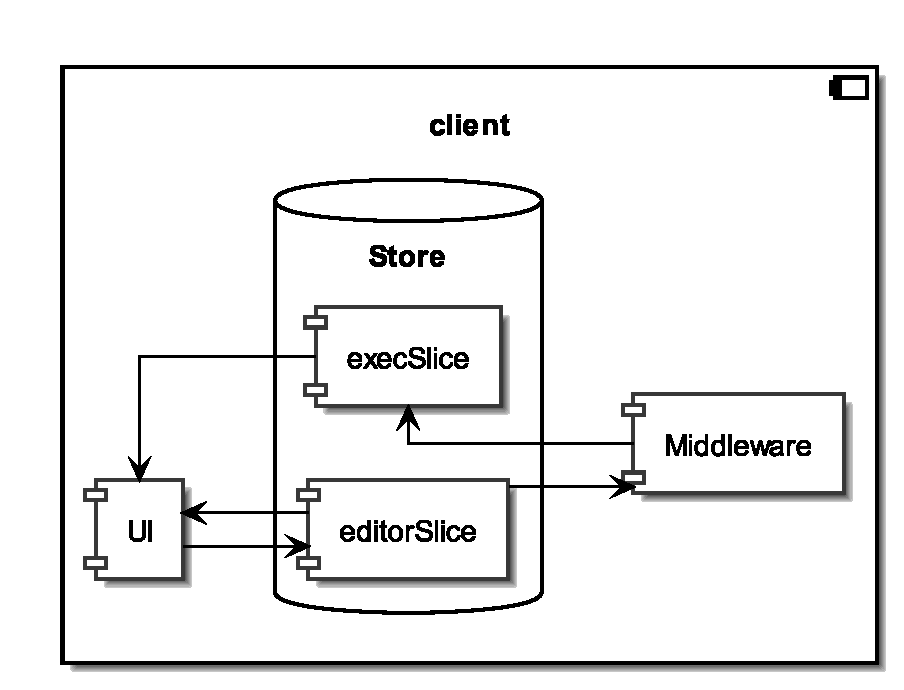
\includegraphics[width=.9\textwidth]{res/uml/architecture-design-client.eps}
          \end{figure}
        \end{column}
      \end{columns}

      % \begin{figure}
      %   \centering
      %   \only<2>{%
      %     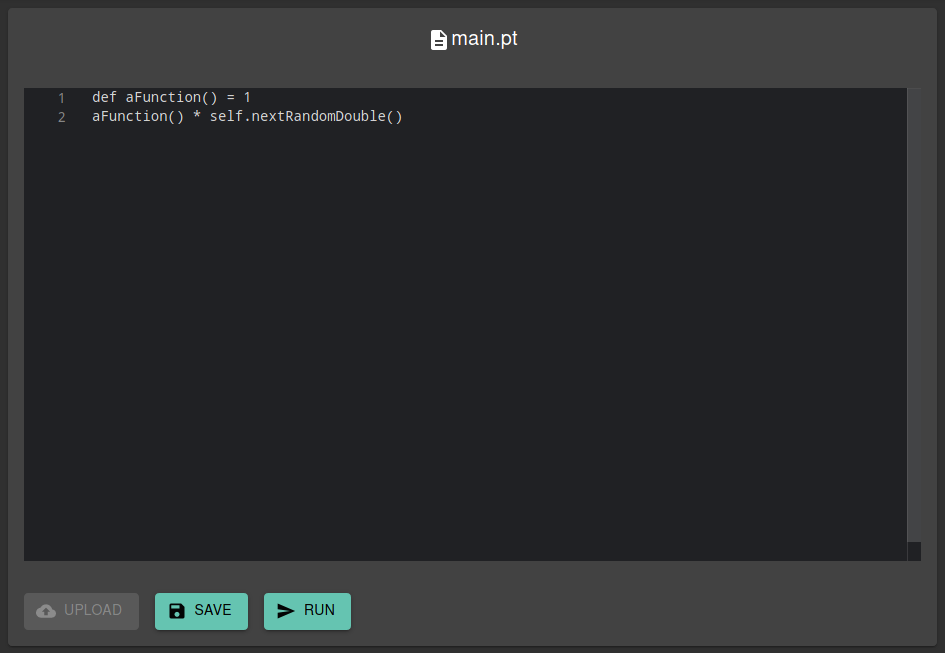
\includegraphics[width=.65\textwidth]{../res/screenshot/Screenshot_2020-03-02 Protelis on the Web(2).png}%
      %   }%
      %   \only<3>{%
      %     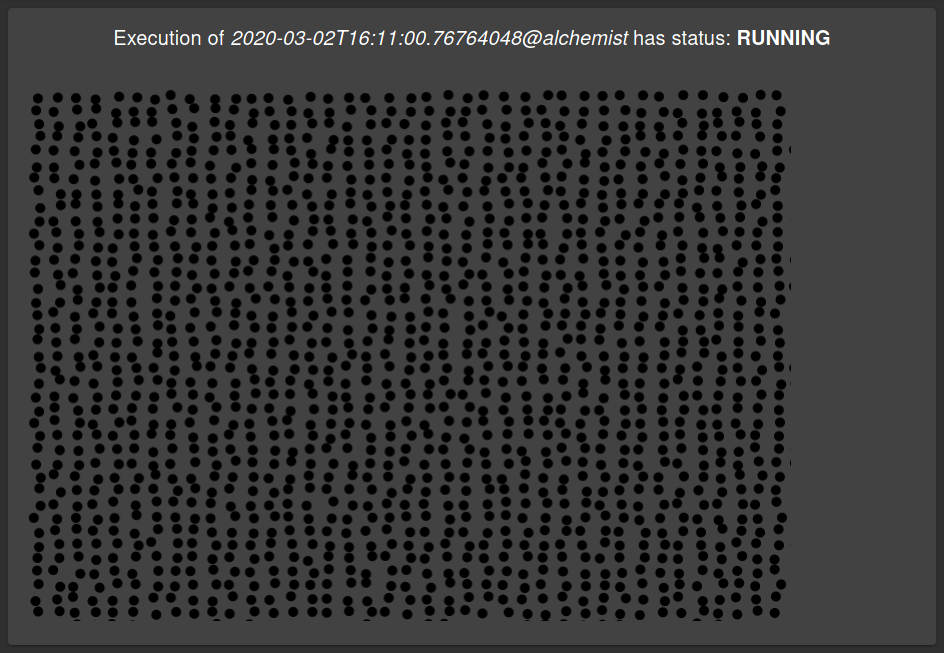
\includegraphics[width=.65\textwidth]{../res/screenshot/Screenshot_2020-03-02 Protelis on the Web(7).png}%
      %   }%
      % \end{figure}
    \end{frame}

  \subsection{Valutazione dei risultati}

    \begin{frame}{\insertsectionhead}{\insertsubsectionhead{}: Demo}
      \centering
      \includemedia[%
        width=.9\textwidth,%
        height=.35\textwidth,%
        keepaspectratio,%
        activate=onclick,%
        deactivate=pageclose,%
        passcontext,%
        transparent,%
        addresource=res/demo.mp4,%
        flashvars={source=res/demo.mp4}%
      ]{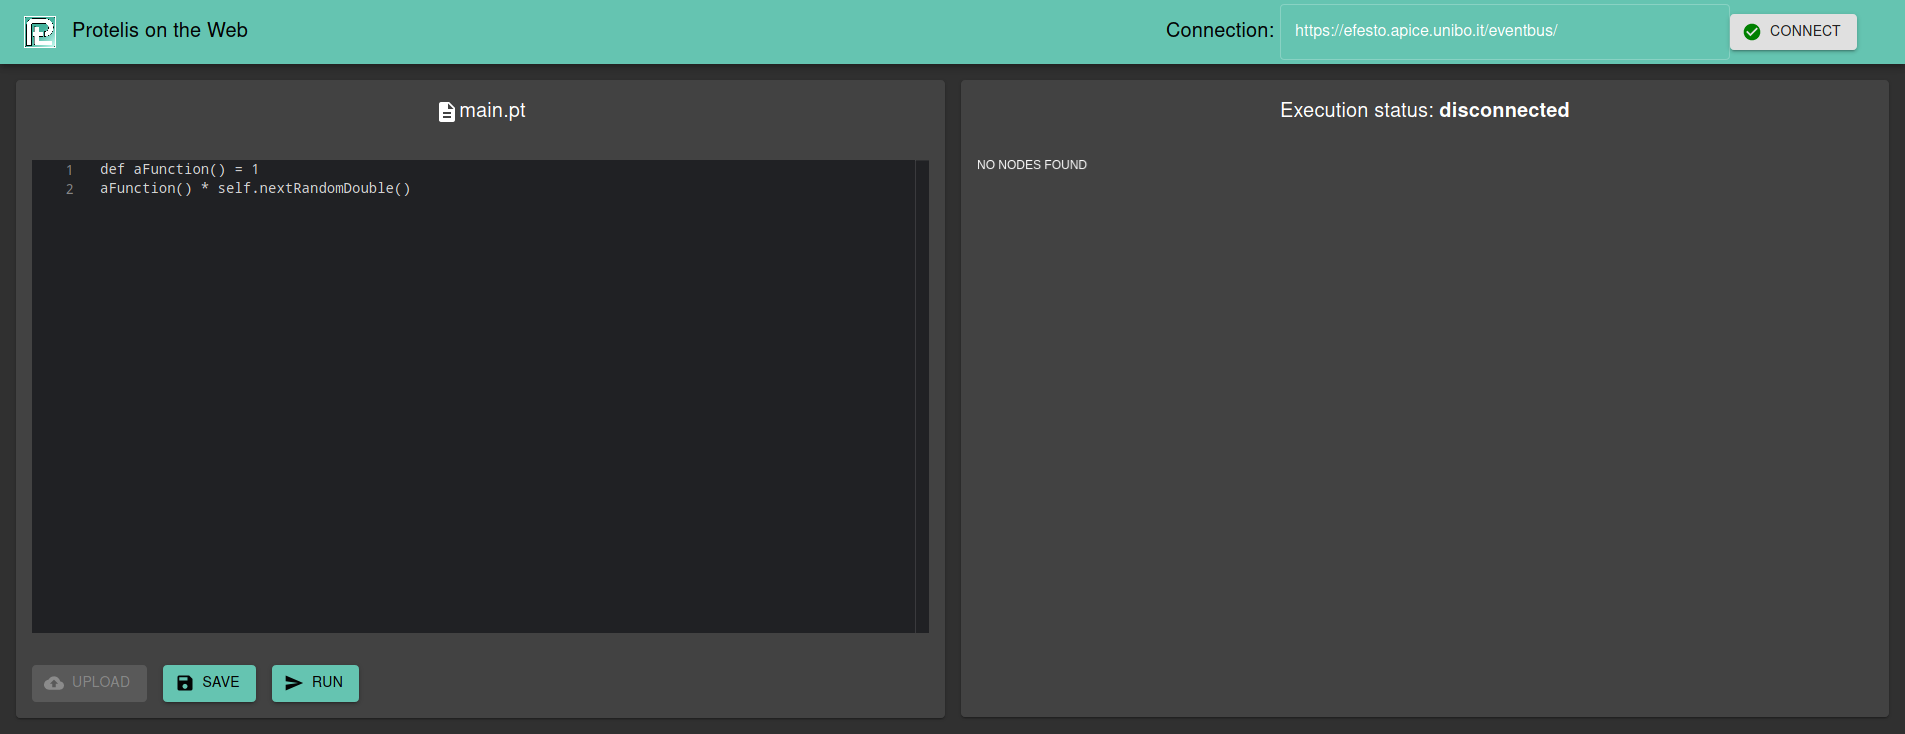
\includegraphics[width=.9\textwidth]{../res/screenshot/Screenshot_2020-03-02 Protelis on the Web(1).png}}{VPlayer.swf}
    \end{frame}

    \begin{frame}{\insertsectionhead}{\insertsubsectionhead{}: Google Lighthouse}
      \centering
      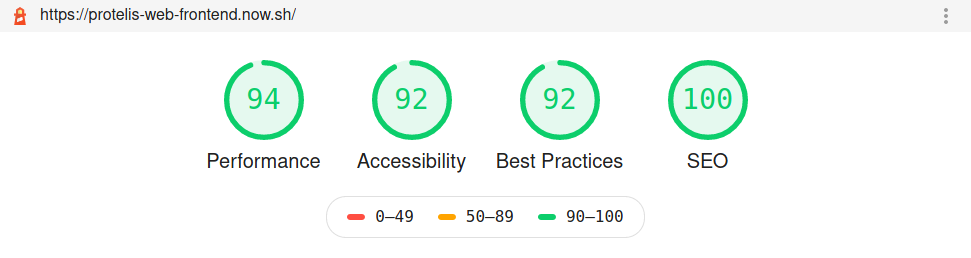
\includegraphics[width=\textwidth]{../res/tests/Screenshot_2020-03-04 Lighthouse Report Viewer.png}
    \end{frame}


  \chapter{Considerazioni finali}\label{ch:considerations}
  % TODO

  % L'obiettivo di questa tesi era quello di realizzare un'interfaccia grafica per l'ambiente di
  % simulazione di Alchemist che sostituisse la precedente e si andasse ad integrare con i recenti
  % contributi dati ad altre sezioni della GUI del software, andando a fornire una esperienza
  % utente più semplice e gradevole anche per i meno esperti.
  % L'interfaccia, realizzata con la libreria JavaFX, ha comportato un restyling completo
  % a livello estetico e una reimplementazione di numerose parti del codice. Al termine del
  % lavoro illustrato in questa tesi, essa risulta essere in grado di caricare una simulazione,
  % rappresentarla a schermo attraverso effetti importabili ed esportabili per mezzo di file JSON
  % e controllarne il flusso d'esecuzione; l'impatto sulle performance di simulazione rispetto a
  % un'esecuzione headless è accettabile e comparabile con l'interfaccia precedente.
  % Nonostante il lavoro svolto abbia portato a un software correttamente funzionante, la
  % nuova interfaccia grafica non può ancora sostituire completamente quella classica sul canale
  % stabile a causa del mancato supporto ad ambienti con mappe di sfondo, del quale non è
  % stato intrapreso lo sviluppo in quanto la mole di lavoro necessaria non avrebbe permesso
  % di mantenere i livelli attuali di ottimizzazione e stabilità.
  % Nel paragrafo successivo sono illustrati i lavori futuri che possono essere apportati per
  % rendere la GUI utilizzabile nel ramo stabile.


  % \frame{\titlepage}

\end{document}
